\documentclass[10pt]{jarticle}
\usepackage{ascmac}
\usepackage[dvipdfmx]{graphicx}
\usepackage{enumerate}
\usepackage{url}
\usepackage{listings}
\usepackage[hang,small,bf]{caption}
\usepackage[subrefformat=parens]{subcaption}
\renewcommand{\lstlistingname}{source}
\lstset{language=sh,%
        basicstyle=\footnotesize,%
	commentstyle=\textit,%
	classoffset=1,%
	keywordstyle=\bfseries,%
	frame=shadowbox,framesep=4pt,%
	showstringspaces=false%,
	numbers=left,stepnumber=1,numberstyle=\footnotesize,%
	numbersep=1zw,%
	lineskip=-0.5ex,%
	xleftmargin=2zw%
	}%

\newdimen\paperwidth \newdimen\paperheight
\def\A4size{\paperwidth=210mm \paperheight=297mm}
\def\centered{%
  \oddsidemargin=\paperwidth
  \advance\oddsidemargin-\textwidth
  \oddsidemargin=0.5\oddsidemargin
  \advance\oddsidemargin-1in
  \evensidemargin-\oddsidemargin}
%
\textwidth 160mm
\textheight 230mm
\topmargin 0mm
\headheight 0mm
\footskip 0mm
\A4size\centered

\title{\framebox{\hspace{4zw}ソフトウェア工学 レポート2%
                 \hspace{4zw}}}
\author{神野　友哉 \\
        2022311042  \\
        愛知県立大学 情報科学部 情報科学科}
\date{2024年7月14日}


\begin{document}

\maketitle

\section{概要} \label{sec:hajime}
レポート\ 1\ で作成したプログラムを現在の\ Java\ の書き方に改良したコードと、
\ Composite\ パターンを適用したコードも作成し、それらの出力が互いに変わらないこと、及び、
後者が前者と比較して保守性を向上していることを考察した。

\section{目的} \label{sec:mokuteki}
クラス間連携に適した構造を理解すること、
それに加えて、簡潔で保守性の高いコードを書けるようになること。

\section{方法} \label{sec:houhou}
レポート\ 1\ で作成したパターン未適用の各クラスのコードを、今風な\ Java\ の書き方に変更した
クラスがソースコード\ref{s1}～\ref{s5}\ CityNeo、\ PrefectureNeo、\ RegionNeo、\ CountryNeo、\ SoftwareNotPaternNeo\ となっている。
また、パターン適用した場合のコードはソースコード\ref{s6}～\ref{s9}\ District、\ GroupDistrict、\ UnitDistrict、\ SoftwarePatern\ である。
\ Powershell\ でのコンパイル・実行は、
\begin{itemize}
	\setlength{\leftskip}{7mm}
	\item[前者 : ] \ javac SoftwareNotPaternNeo.java\ \\
		\ java SoftwareNotPaternNeo\ 
	\item[後者 : ] \ javac SoftwarePatern.java\ \\
		\ java SoftwarePatern\
\end{itemize}
である。その際に、ソースコードと同じ階層である必要がある。

\subsection{作成したプログラム}
\lstinputlisting[caption= パターン未適用 CityNeo.java, label=s1]{./java/CityNeo.java}
\lstinputlisting[caption= パターン未適用 PrefectureNeo.java, label=s2]{./java/PrefectureNeo.java}
\lstinputlisting[caption= パターン未適用 RegionNeo.java, label=s3]{./java/RegionNeo.java}
\lstinputlisting[caption= パターン未適用 CountryNeo.java, label=s4]{./java/CountryNeo.java}
\lstinputlisting[caption= パターン未適用 SoftwareNotPaternNeo.java, label=s5]{./java/SoftwareNotPaternNeo.java}
\lstinputlisting[caption= パターン適用 District.java, label=s6]{./java/District.java}
\lstinputlisting[caption= パターン適用 GroupDistrict.java, label=s7]{./java/GroupDistrict.java}
\lstinputlisting[caption= パターン適用 UnitDistrict.java, label=s8]{./java/UnitDistrict.java}
\lstinputlisting[caption= パターン適用 SoftwarePatern.java, label=s9]{./java/SoftwarePatern.java}

\newpage
\section{実験結果} \label{sec:kekka}
図\ref{fig:kekka2}から、パターン未適用と適用した場合を比較しても、
デバッグ出力に違いは見られなかった。
\begin{figure}[htbp]
	\begin{center}
		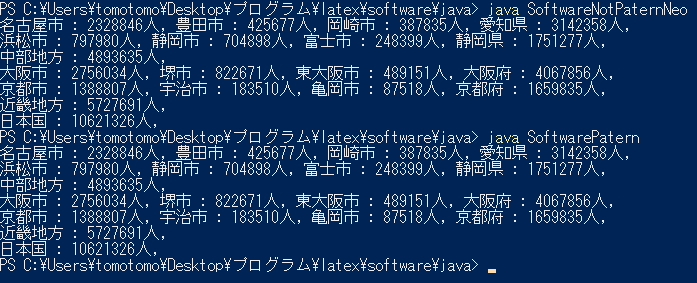
\includegraphics[width=100mm]{kekka2.png}
	\end{center}
	\caption{動作確認用のデバッグ出力}
	\label{fig:kekka2}
\end{figure}

\section{考察}
\subsection{課題 3 その他、モダンな Java に書き換えよ}
\begin{lstlisting}[caption=レポート1 課題2 Prefecture.java getPopulation() 所属市人口加算部分,label=lst:for]
	int result = 0;
	for (int i = 0; i < cities.size(); i++) {
		City city = (City) cities.get(i);
		result += city.getPopulation();
	}
\end{lstlisting}
\begin{lstlisting}[caption=レポート2 課題3 PrefectureNeo.java getPopulation() 所属市人口加算部分,label=lst:stream]
	int result = cities.stream()
			.mapToInt(CityNeo::getPopulation)
			.sum();
\end{lstlisting}
パターン未適用のコードにおいて、\ Stream\ API\ を用いて\ ArrayList\ の全要素の人口を合算した値を計算する方式に変更した。
それは、県の人口計算処理部分における、変更前コード\ref{lst:for}と変更後コード\ref{lst:stream}から
その処理を実装するコードが更に簡潔にまとまっていることが判る。そのため、可読性や保守性の向上に貢献していると考えられる。余談だが、
変更前コード\ref{lst:for}に (City) とあるが、\ ArrayList\ に\ Generics\ を適用しているため、キャストは必要なかったことが判る。
\subsection{課題 4 Composite デザインパターンを適用し、適用前との相違を比較せよ}
動作やデバッグ出力は課題\ 3\ で作成したパターン未適用のコードと同様の仕様にした。それは、実験結果\ref{sec:kekka}からも明らかである。
同じ結果となるように実装した二つのコードの好ましさについて検証したい。
ソースコード\ref{s1}～\ref{s9}から、
コードの記述量やクラスの数の削減、各クラスで共通に存在する似たような処理を\ abstract\ クラスで部分的に実装して
いるという相違点から、\ Composite\ デザインパターンを適用した方が、前述した可読性や保守性の観点から、好ましいと考えられるのではないか。

\section{感想}
\ Stream\ API\ を用いる前、拡張\ for\ 文で一度実装していた。なぜなら、\ forEach(Consumer c)\ での
実装を試みたが、\ Consumer\ は戻り値がないため、人口を戻り値とする\ getPopulation\ メソッドを
実引数として入れることが出来なかった。\ forEach\ 内での外部変数の変更は却って複雑になっているように感じたため
\ Stream\ API\ の\ mapToInt\ と\ sum\ メソッドを用いることとした。
\begin{lstlisting}
	int result = 0;
	for (City city : cities) result += city.getPopulation();
\end{lstlisting}
\begin{lstlisting}
	AtomicInteger result_a = new AtomicInteger(0);
	cities.forEach(city -> result_a.addAndGet(city.getPopulation()));
	int result = result_a.get();
\end{lstlisting}

\end{document}
